\documentclass[11pt,a4paper]{article}
\usepackage[utf8]{inputenc}
\usepackage{amsmath}
\usepackage{amsfonts}
\usepackage{amssymb}
\usepackage{tikz}
\author{Mikkel Riber Bojsen - s093255}
\begin{document}
\section{$\mathcal{NP}$-completeness}

To prove $\mathcal{NP}$-completeness, we look at the problem \textsc{PartitionByPairs} (PBP). 

\subsection{Transformation}
Given an instance of PBP $X$, we do the following transformation. We calculate the value $B = \frac{\sum_{i=1}^{2n} s_i}{2}$. For each pair in $S$, $(s_{2i-1}, s_{2i})$ where $i \in \lbrace 1,\dots, n \rbrace $, we construct a graph as show in Fig.~\ref{fig:transform1}, where the labels are the weights of the corresponding edge. 

\begin{figure}[!htb]
\centering
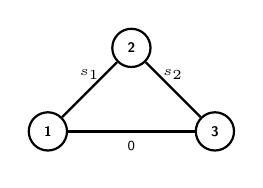
\begin{tikzpicture}[auto,node distance=1.5cm,
  thick,main node/.style={circle,draw,font=\sffamily\tiny\bfseries}]

  \node[main node] (1) {1};
  \node[main node] (2) [above right of=1] {2};
  \node[main node] (3) [below right of=2] {3};
 % \node[main node] (4) [right of=3] {4};

  \path[every node/.style={font=\sffamily\tiny}]
    (1) edge node [above] {$s_1$} (2)
    	edge [right] node [below] {0} (3)
    (2) edge node [above] {$s_2$} (3);
    %	edge [bend left] node {0} (4)
   % (3) edge node {$s_2$} (4);

\end{tikzpicture}
\caption{Transformation of a single pair}
\label{fig:transform1}
\end{figure}

We order the edges so the mirror of the edge with weight $s_{2i-1}$ is $s_{2i}$ and the mirror of an edge with weight 0 is an edge with weight 0. For multiple pairs, we chain multiple pairs together as shown in Fig.~\ref{fig:transform2}. For example, the edge weight distribution for $S={1,2,3,4,5,6}$, the weights will be distributed  as $w(e_i) = i$ for $i\in \lbrace 1,3,5,0,0,0,B,B,B,0,0,0,6,4,2 \rbrace$. 

\begin{figure}[htb]
\resizebox{\linewidth}{!}{
\centering
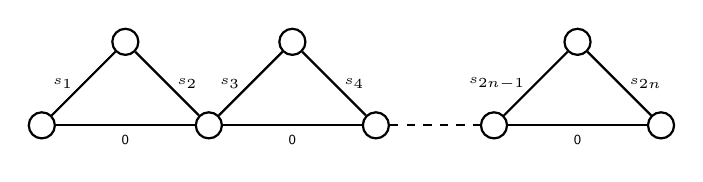
\begin{tikzpicture}[auto,node distance=1.5cm,
  thick,main node/.style={circle,draw,font=\sffamily\small\bfseries}]

  \node[main node] (1) {};
  \node[main node] (2) [above right of=1] {};
  \node[main node] (3) [below right of=2] {};
  \node[main node] (4) [above right of=3] {};
  \node[main node] (5) [below right of=4] {};
  \node[main node] (6) [right of=5] {};
  \node[main node] (7) [above right of=6] {};
  \node[main node] (8) [below right of=7] {};


  \path[every node/.style={font=\sffamily\tiny}]
    (1) edge node [left] {$s_1$} (2)
    	edge [right] node [below] {0} (3)
    (2) edge node [right] {$s_2$} (3)
    
     (3) edge node [left] {$s_3$} (4)
        	edge [right] node [below] {0} (5)
        (4) edge node [right] {$s_4$} (5)
    	
     (6) edge node [left] {$s_{2n-1}$} (7)
        	edge [right] node [below] {0} (8)
        (7) edge node [right] {$s_{2n}$} (8)
        
        ;
             
   \draw[style=dashed, ] (5) -- (6);
\end{tikzpicture}}
\caption{Graph of several pairs}
\label{fig:transform2}
\end{figure}

Using this graph and the calculated value $B$ we can query MFMST.

\subsection{Proof}

We do our transformation in polynomial time. The calculation of $B$ is done in $O(n)$. For each pair, we construct a constant number of nodes and edges in constant time, so the graph can be created in $O(n)$, this means our transformation can be done in $O(n)$.

If the answer to the original problem instance $X$ is YES, it means that a partition where we pick one from each pair equals $B$. It is possible to pick a spanning tree where we pick one from each pair as shown in Fig~\ref{fig:transform3}

\begin{figure}[htb]
\resizebox{\linewidth}{!}{
\centering
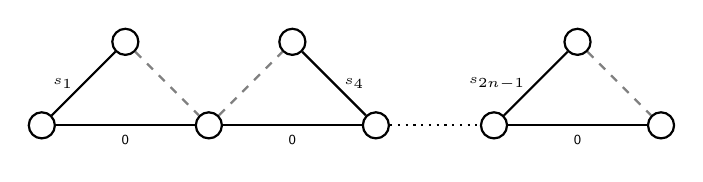
\begin{tikzpicture}[auto,node distance=1.5cm,
  thick,main node/.style={circle,draw,font=\sffamily\small\bfseries}]

  \node[main node] (1) {};
  \node[main node] (2) [above right of=1] {};
  \node[main node] (3) [below right of=2] {};
  \node[main node] (4) [above right of=3] {};
  \node[main node] (5) [below right of=4] {};
  \node[main node] (6) [right of=5] {};
  \node[main node] (7) [above right of=6] {};
  \node[main node] (8) [below right of=7] {};


  \path[every node/.style={font=\sffamily\tiny}]
    (1) edge node [left] {$s_1$} (2)
    	edge [right] node [below] {0} (3)
   % (2) edge node [right] {$s_2$} (3)
    
     (3) % edge node [left] {$s_3$} (4)
        	edge [right] node [below] {0} (5)
        (4) edge node [right] {$s_4$} (5)
    	
     (6) edge node [left] {$s_{2n-1}$} (7)
        	edge [right] node [below] {0} (8)
   %     (7) edge node [right] {$s_{2n}$} (8)
        
        ;
             
   \draw[style=dotted, ] (5) -- (6);
    \draw[color=gray, dashed] (2) -- (3);
        \draw[color=gray, dashed] (3) -- (4);
            \draw[color=gray, dashed] (7) -- (8);
\end{tikzpicture}}
\caption{A spanning tree}
\label{fig:transform3}
\end{figure}

\end{document}